\section{Introduction}

%
% Thanks to Martha Field for discussion on adapting mammalian cells
% to synthetic media.
%
FBA (flux balance analysis) is the oldest, simplest, and perhaps
most widely used linear constraint-based metabolic modeling approach
\citep{Shestov2013a,Lewis2012}. FBA has become extremely popular, in
part, due to its simplicity in calculating reasonably accurate
microbial fluxes or growth rates
(e.g.\ \citealt{Schuetz2012,Fong2004_sb2013}); for
many microbes, a simple synthetic environment where all chemical
species are known suffices to allow proliferation, giving fairly
complete constraints on model inputs. Additionally, it has been found
that their biological objectives can be largely expressed as linear
objectives of fluxes, such as maximiztion of biomass \citep{Schuetz2012}. 
Neither of these assumptions necessarily hold for mammalian cells growing \textit{in
  vitro} or \textit{in vivo}, and in particular the environment is far
more complex for mammalian cell cultures, which have to undergo
gradual metabolic adaptation via titration to grow on synthetic media
\citep{Pirkmajer2011}. Recently, there have been many efforts to
incorporate both absolute and differential expression data into
metabolic models \citep{Blazier2012}. The minimization of metabolic
adjustment (MoMA) algorithm is the simplest metabolic flux fitting
algorithm, and it can be extended in order to allow the use of
absolute expression data for the estimation of flux as in FALCON
\citep{Segre2002,Lee2012}.

% May eventually want to make this a conditional include section
% and include it earlier in dissertation.
%\subsection{MoMA: Minimization of Metabolic Adjustment}

The MoMA method is framed as a constrained least-squares optimization
problem, is typically employed to calculate the flux vector of an
\textit{in silico} organism after a mutation by minimizing the distance
between the wild-type flux and the mutant flux. The biological
intuition is that the organism has not had time to adapt to the
restricted metabolic capacity and will maintain a similar flux to the
wild-type (WT) except where the perturbations due to the mutation
dictate necessary alterations in fluxes \citep{Shlomi2005}. Suppose
$\mathbf{a}$ is the WT flux vector obtained by an optimization
procedure such as FBA, empirical measurements, or a combination of
these. For an undetermined flux vector $\mathbf{v}$ in a model with
$N$ reactions the MoMA objective can be expressed as
\[ \textnormal{minimize}\ \sum\limits_{i=1}^N (v_i-a_i)^2 \] 
subject to the stoichiometric constraints $\mathbf{S v}\nolinebreak
=\nolinebreak \mathbf{0}$ where $\mathbf{v} = (v_1, \ldots,
v_N)^T$ and $\mathbf{S}$ is the stoichiometric matrix (rows correspond
to metabolites, columns to reactions, and entries to stoichiometric
coefficients). Constant bounds on fluxes are often present, such as
substrate uptake limits, or experimental $V_{\max}$ estimates, so we
write these as the constraints $\mathbf{v}_{lb}\nolinebreak
\preceq\nolinebreak \mathbf{v}\nolinebreak \preceq \mathbf{v}_{ub}$.
The objective may be equivalently expressed in the canonical
quadratic programming (QP) vector form as
$\textnormal{min.\ }\ \frac{1}{2}\mathbf{v}^T \mathbf{v}\nolinebreak
-\nolinebreak \mathbf{a}^T \mathbf{v}$. This assumes that each $a_i$
is measured, but it is also possible and sometimes even more useful to
employ this objective when only a subset of the $a_i$ are measured (if
$a_i$ is not measured for some $i$, then we omit $(v_i-a_i)^2$ from
the objective). In metabolomics, for instance, it is always the case
in experiments with labeled isotope tracers that only a relatively
small subset of all fluxes are able to be estimated with metabolic
flux analysis (MFA; \citealt{Shestov2013a}). Combining MoMA with MFA
provides a technique to potentially estimate other fluxes in the
network.

A variant of MoMA exists that minimizes the absolute value of the
difference between $a_i$ and $v_i$ for all known $a_i$. To our
knowledge, the following linear program is the simplest version of
linear MoMA, which assumes the existence of a constant flux vector
$\mathbf{a}$ and is expressed as the following linear program:

\begin{center}
\begin{tabular}{rl}
minimize & $\sum\limits_{i=1}^N d_i$  \\
subject to & $\mathbf{S v} = \mathbf{0}$ \\
 & $\mathbf{v}_{lb} \preceq \mathbf{v} \preceq \mathbf{v}_{ub}$ \\
$\forall i:$ & $-d_i \le v_i-a_i \le d_i$ \\
 & $d_i \ge 0$
\end{tabular}
\end{center}

The $d_i$ are just the distances from \textit{a priori} fluxes to
their corresponding fitted fluxes.  Linear MoMA has the advantage that
it is not biased towards penalizing large magnitude fluxes or
under-penalizing fluxes that are less than one
\citep{Boyd2004,Shlomi2005}. Additionally, linear programs are often
amenable to more alterations that maintain convexity than a quadratic
program \citep{Boyd2004}.

If we wish to apply MoMA to expression data rather than flux data, there
are two primary problems that must be tackled. First, we must quantify
enzyme complex abundance as accurately as possible given the gene expression
data. Although there is not a one-to-one correspondence between
reactions and enzyme complexes, the correspondence is much closer
than that between individual genes and metabolic reactions. In the
first part of this work, we describe an algorithm that can account for
enzyme complex formation and thus quantify enzyme complex
abundance. Next, we build on the original MoMA objective, which must
be altered in several ways (also discussed in \citealt{Lee2012} which
lays the groundwork for the current method). We automatically scale
expression values so that they are comparable to flux units obtained
in the optimization routine, which can be an advantage over the prior
method. Also, expression data has no directionality, necessitating
reaction direction assignment in order to compare enzyme complex
abundance and flux directly in the optimization problem
\citep{Lee2012}.  Finally, we employ several sensitivity analyses and
performance benchmarks so that users of the FALCON method and related
methods may have a better understanding of what to expect in practice.

\section{Methods}

Most genome-scale models have attached Boolean (\textit{sans}
negation) gene rules to aid in determining whether or not a gene
deletion will
completely disable a reaction. These are typically called GPR
(gene-protein-reaction) rules and are a requirement for FALCON; their
validity, like the stoichiometric matrix, will undoubtedly be
important for generating accurate predictions. Also important are the
assumptions and limitations for the process of mapping expression data
to complexes so that a scaled enzyme complex abundance (hereafter
referred to as complex abundance) can be estimated. We address these
in the next section and have attached a flow chart to illustrate the
overall process of mapping expression of individual genes to enzyme
complexes within the greater context of flux estimation 
(\textbf{Fig.~\ref{ECCN_flowchart}}). We develop an algorithm for
this step---finding the minimum disjunction---for estimating complex
abundance as efficiently and as accurately as possible given the
assumptions (due primarily to limitations in data quality; \suppOrApp
Section~\ref{sec:complexation}).

%\vspace{5 mm} 
\begin{figure}
\centering
\begin{tikzpicture}%[scale=0.8, node distance = 1cm, auto]
    % Place nodes
    \node [block] (start) {start}; 
    \node [iogram, below of=start, left of=start] (exp) {Genes:\\ expression 
      ($\mu$,~$\sigma$)}; 
    \node [iogram, below of=start, right of=start] (rules) {Reactions:
      GPR Rule}; 
    \node [block, below of=rules] (parse) {Parse Rule}; 
    \node [block, below of=parse, left of=parse, xshift=-0.5cm]
      (mindisj) {Find minimum disjunction};
    \node [iogram, below of=mindisj] (expstd)
          {Reactions (enzyme~complexes):\\ abundance ($\mu$,~$\sigma$)};
    \node [iogram, right of=falcon, below of=expstd] (smat) 
      {$\mathbf{S}$ matrix};
    \node [iogram, left of=falcon, below of=expstd] (vbnd) 
      {Reactions:\\ flux bounds ($\mathbf{v}_{lb}$, $\mathbf{v}_{ub}$)};
    \node [block, below of=vbnd, left of=smat, right of=vbnd, 
      below of=expstd, yshift=-0.5cm] (falcon) 
      {Flux fitting (FALCON)};
    \node [iogram, below of=falcon] (fluxout) 
      {Reactions:\\ fluxes ($\mathbf{v}:$ $\mu$,~$\sigma$)};
    % Draw edges
    \path [line] (start) -- (exp);
    \path [line] (start) -- (rules);
    \path [line] (rules) -- (parse);
    \path [line] (exp.south) -- (mindisj);
    \path [line] (parse) -- (mindisj);
    \path [line] (mindisj) -- (expstd);
    \path [line, transform canvas={xshift=0.25cm}] (expstd) -- (falcon);
    \path [line] (rules.east) |- (falcon.east);
    \path [line] (smat) -- (falcon);
    \path [line] (vbnd) -- (falcon);
    \path [line] (falcon) -- (fluxout);

\end{tikzpicture}
\caption{Flowchart illustrating the two algorithms presented in this
paper. The process of estimating enzyme complex abundance is displayed
in detail, whereas the flux-fitting algorithm (FALCON) is illustrated
as a single step for simplicity. First, for each gene in the model
with available expression data, the mean and (if available) standard
deviation or some other measure of uncertainty are read in. Gene rules
(also called GPR rules) are also read in for each enzymatic
reaction. The reaction rules are parsed and the minimum disjunction
algorithm (Algorithm~\ref{alg:ReductionToCNF}) is applied, making use
of the gene's mean expression. Next, the estimated and unitless enzyme
complex abundance and variance are output for each enzymatic
reaction. Finally, flux fitting with FALCON
(Algorithm~\ref{alg:FALCON}) can be applied, and requires the model's
stoichiometry and flux bounds. The final output has the option of
being a deterministically estimated flux, or a mean and standard
deviation of fluxes if alternative optima are explored.}
\label{ECCN_flowchart}
\end{figure}

\subsection{Estimating enzyme complex abundance}

Given the diversity and availability of genome-scale expression datasets,
either as microarray or more recently RNA-Seq, it could be useful to
gauge the number of enzyme complexes present in a cell. A recent
study found that only 11\% of annotated \textit{Drosophila}
protein complexes have subunits that are co-expressed
\citep{Juschke2013}, so it cannot be assumed that any given protein
subunit level represents the actual complex abundance. We formalize a
model for enzyme complex formation based on GPR rules that are
frequently available in genome-scale annotations.

The original expression to complex abundance mapping procedure
performed a direct evaluation of GPR rule expression
values---replacing gene names with their expression values, ANDs with
minimums, and ORs with sums, without altering the logical expression
of the GPR rule in any way \citep{Lee2012}. Below we illustrate a 
problem that can occur with this mapping where some genes' expression
levels may be counted more than once. 

The $r_i$ are different reaction rules and the $e_i$ are the
corresponding estimated complex abundance levels. Lower case letters
are shorthand for the expression level of the corresponding gene ID in
uppercase; for example, $a = \E{\textnormal{A}}$, where
$\E{\textnormal{A}}$ is the expression of gene A.

\begin{AlgFloat}[H]
{\setlength{\tabcolsep}{.16667em}
\begin{tabular}{cccccccc}
& $r_1$ & := & [A and B] or [A and C] & $\rightarrow$ & $e_1$  &=& $\min(a,b$) + $\min(a,c$) \\ 
& $r_2$ & := & [A and (B or C)]       & $\rightarrow$ & $e_2$  &=&  $\min(a, b + c$) 
\end{tabular} 
}
\end{AlgFloat}
%Really we should be testing for number of text columns:
%\ifthenelse{\boolean{thesisStyle}}{\ruleEx1}{\hspace*{-4em}{\ruleEx1}} 

Supposing A is the minimum, then if we just evaluate $r_1$ directly (a
rule in disjunctive normal form, or DNF), A will be counted twice.
Rules with sub-expressions in DNF are frequently encountered in practice,
but directly evaluating them can lead to erroneous quantification.

Another possibility is partitioning expression among multiple occurrences
of a gene in a rule. For instance, in $r_1$ above, we could evaluate
it as $e_1$ =
min($\frac{a}{2},b$) + min($\frac{a}{2},c$) to account for the
repeated use of $a$. However, other potential issues aside, we can see
that this can cause problems rather quickly. For instance, suppose $b
= a$ and $c = 0$; then min($a$,$b+c$) $=b=a$ appears to be correct,
not min($\frac{a}{2},b$) + min($\frac{a}{2},c$) = $\frac{a}{2} + 0$.
From this example, we can see that conversion to conjunctive normal
form (CNF) appears to be a promising prerequisite for evaluation.

\subsection{The min-disjunction algorithm estimates \\enzyme complex abundance}

In the \suppOrApp (Section~\ref{sec:complexation}), we show that
converting a rule to CNF is a sound method
to aid in the estimation of enzyme complex abundance. We use a
reduction rule that removes redundant genes from the complex
(e.g. holoenzymes; see \suppOrApp Assumption~\ref{asm:holo}), outlined
below. This effectively finds the \emph{rate-limiting} component of
enzyme-complex formation. The algorithm can be described \hl{as follows:}


Although conversion to CNF may be intractable for some rules
\citep{Russell2009}, we tested our implementation of the algorithm on
three of the most well-curated models which likely contain some of the
most complex gene rules available. These models are for \textit{E. coli}
\citep{Orth2011a}, yeast \citep{Aung2013}, and human
\citep{Thiele2013}. In all cases, the rules were converted to CNF in
less than half a second, which is far less than the typical flux
fitting running time from Algorithm~\ref{alg:FALCON}. We also present
a heuristic algorithm (Section~\ref{sec:HeuristicToCNF}) that should
work quickly even on rules that are not able to be strictly converted
to CNF, and in most cases should still yield the minimum disjunction.

Application of Algorithm~\ref{alg:ReductionToCNF} results in several
differences from direct substitution and evaluation in yeast GPR
rules. When data completely covers the genes in the model
(e.g. \citealt{Lee2012}), rules tend to have few differences in Yeast
regardless of the evaluation method (25 rules; 1.08\% of all rules for
Yeast 7). This number goes up significantly in Human Recon 2
\citep{Thiele2013} due to more complex GPR rues (935 rules; 22\% of
all rules). For the human model, we could not find any data set that
covered every gene, so instead random expression data roughly matching
a power law was used to generate this statistic. If we use proteomics
data for yeast and human models, the difference in how missing gene
data is handled causes some additional increase in differences
\citep{Picotti2013,Gholami2013}.  For proteomics, in the Yeast 7 model
205 rules (8.87\% of all rules) differed, and in Human Recon 2, 1002
rules (23.57\% of all rules) differed. We can see that in Yeast, the
changes in flux attributed to enzyme abundance evaluation can be
relatively small for data with 100\% gene coverage, but the other
extreme in Human can be significant (\textbf{Figure EnzAbundEval}).

%
% Above, to make the figure more striking, we can say that if we
% don't include the information about the missing results, we
% maintain a constant 10% (which thus reverses the wording in a sense).
%


\subsection{Formulation with automatic normalization and batch direction assignment}

Prior work that served as an inspiration for this method used Flux
Variability Analysis (FVA) to determine reaction direction
\citep{Lee2012}. Briefly, this involves two FBA simulations per
reaction catalyzed by an enzyme, and as the algorithm is iterative,
this global procedure may be run several times before converging to a
flux vector. We removed FVA to mitigate some
of the cost, and instead assign flux direction in batch; while it is
possible that the objective value may decrease using this approach,
this is not an issue since the objective function increases to include
more irreversible fluxes at each iteration, and the objective value of
a function with more fluxes should supersede the importance of one
with fewer fluxes.
 
To make working with irreversible fluxes simpler, we convert the model
to an irreversible model, where each reversible flux $v_j$ in the
original model is split into a forward and a backward reaction that take
strictly positive values: $v_{j,f}$ and $v_{j,b}$. If $v_j$ is
specified without a forward or backward subscript and it is in the
context of an irreversible model, this implies that the reaction
direction is irreversible. We also account for enzyme complexes
catalyzing multiple reactions by including all reactions with identical
GPR rules in the same residual
constraint; indexed sets of reactions are denoted $R_i$ and their
corresponding estimated enzyme abundance is $e_i$. \textbf{Figure FalconGrp} 
shows the difference in Algorithm~\ref{alg:FALCON} when we do not 
use reaction group information. Note that we use a
slight abuse of notation, since we also choose to index enzyme
abundance as $e_j$ for a specific reaction, where $j = i$ does not
imply $e_i = e_j$. The \emph{existence} of $e_j$ merely means that
some expression data is available for some of the genes for $e_j$;
missing genes are removed from the rule during the call to
min-disjunction---values known to be zero can always be specified as
such. The standard deviation of enzyme abundance, $\sigma_i$, is an
optional weighting of uncertainty in biological or technical
replicates.

We employ a normalization variable $n$ in the problem's objective and
flux-fitting constraints to find the most agreeable scaling of
expression data. The linear fractional program shown below can be
converted to a linear program by the Charnes-Cooper transformation
\citep{Boyd2004}. To avoid the need for fixing any specific flux, which
may introduce bias, we introduce the bound $\sum_{j \mid e_j 
\textnormal{ exists }} v_j \geq V_{lb}^{\Sigma}$. This guarantees that
the optimization problem will yield a non-zero flux vector. As an
example of how this can be beneficial, this means we do not need to
measure any fluxes or assume a flux is fixed to achieve good results;
though this does not downplay the value of obtaining
experimentally-based constraints on flux when available 
(\suppOrApp Fig.~\ref{fig:FluxBars}).

Algorithm~\ref{alg:FALCON} and the method in \citealt{Lee2012} are
both non-deterministic. In the first case, Algorithm~\ref{alg:FALCON}
solves an LP during each iteration, and subsequent iterations depend
on the LP solution, so that alternative optima may affect the outcome.
In the latter case, alternative optima of individual LPs is not an
issue, but the order in which reactions assigned to be irreversible can
lead to alternative solutions. However, we
found that the variation due to this stochasticity is typically 
relatively minor, particularly in cases where the model is more 
heavily constrained (\suppOrApp Fig.~\ref{fig:FluxBars}; Figure EnzAbundEval).

% Make performance tables like this? 
% Apparently the processtable and rules below are not
% standard latex

%% \begin{table}[!t]
%% \processtable{This is table caption\label{Tab:01}}
%% {\begin{tabular}{llll}\toprule
%% head1 & head2 & head3 & head4\\\midrule
%% row1 & row1 & row1 & row1\\
%% row2 & row2 & row2 & row2\\
%% row3 & row3 & row3 & row3\\
%% row4 & row4 & row4 & row4\\\botrule
%% \end{tabular}}{This is a footnote}
%% \end{table}

%% %\end{methods}

%% \begin{figure}[!tpb]%figure1
%% %\centerline{\includegraphics{fig01.eps}}
%% \caption{Caption, caption.}\label{fig:01}
%% \end{figure}

%% \begin{figure}[!tpb]%figure2
%% %\centerline{\includegraphics{fig02.eps}}
%% \caption{Caption, caption.}\label{fig:02}
%% \end{figure}

\section{Results and Discussion}

\subsection{Performance benchmarks}
Using the same yeast exometabolic and expression data employed for
benchmarking in the antecedent study \citep{Lee2012} that included an
updated version of the Yeast 5 model \citep{Heavner2012} and the latest
Yeast model \citep{Aung2013}, we find that
our algorithm has significant improvements in time efficiency while
maintaining correlation with experimental fluxes, and is much faster 
than any similarly performing method (Table~\ref{tab:FalcPerf}; 
\suppOrApp Fig.~\ref{fig:FluxBars}).
Timing for the human model also improved in FALCON; in a model with
medium constraints and exometabolic directionality constraints, FALCON
completed on average in 3.6~m and the method from \citealt{Lee2012} in
1.04~h.


\begin{table*}
\begin{center}
\begin{tabular}{rrrrrrrrrr}
%\emph{Model}                 & \emph{Primal-Simplex} & \emph{Dual-Simplex} & \emph{Barrier} \\
\textbf{(a)} \hspace{1.4cm} & Max. $\mu$ & Model & Experimental & 
  Standard FBA & Fitted FBA & GIMME & iMAT & Lee et al & FALCON\\
 & 75 \%& Yeast5 MC & 1 & 0.66 & 0.66 & NaN  & 0.57 & 0.64 & 1 \\
 & 75 \%& Yeast7 MC & 1 & 0.66 & 0.66 & 0.68 & 0.66 & 0.66 & 0.98\\
 & 75 \%& Yeast5 HC & 1 & 0.73 & 0.78 & 0.75 & 0.66 & 0.98 & 0.99\\
Pearson's r  
 & 75 \%& Yeast7 HC & 1 & 0.70 & 0.70 & 0.80 & 0.66 & 0.98 & 0.99\\
 & 85 \%& Yeast7 MC & 1 & 0.62 & 0.62 & 0.65 & 0.62 & 0.62 & 0.97\\
 & 85 \%& Yeast5 HC & 1 & 0.88 & 0.89 & 0.9  & 0.81 & 0.99 & 0.99\\
 & 85 \%& Yeast7 HC & 1 & 0.67 & 0.67 & 0.87 & 0.62 & 0.98 & 0.98\\
\end{tabular}
\begin{tabular}{rrrrrrrrrr}
\textbf{(b)} \hspace{1.4cm} & Max. $\mu$ & Model & Experimental & 
  Standard FBA & Fitted FBA & GIMME & iMAT & Lee et al & FALCON\\
 & 75 \%& Yeast5 MC & 0 & 0.9  & 470   & 0.81  & 50     & 110 & 1.8 \\
 & 75 \%& Yeast7 MC & 0 & 1.9  & 3,100 & 2.1   & 12,000 & 600 & 5.6 \\
 & 75 \%& Yeast5 HC & 0 & 0.12 & 110   & 0.18  & 1.4    & 15  & 0.27\\
Time (s) 
 & 75 \%& Yeast7 HC & 0 & 0.72 & 940   & 1.7   & 240    & 670 & 5.5 \\
 & 85 \%& Yeast7 MC & 0 & 2.3  & 3,100 & 3.8   & 14,000 & 610 & 4.6 \\
 & 85 \%& Yeast5 HC & 0 & 0.12 & 110   & 0.18  & 2.5    & 15  & 0.22\\
 & 85 \%& Yeast7 HC & 0 & 0.70 & 110   & 2.5   & 100    & 530 & 5.9\\
\end{tabular}
\end{center}
\caption{Performance of FALCON and other CBM methods for predicting
yeast exometabolic fluxes \textbf{(a)} and associated timing analysis \textbf{(b)}. For
Lee et al. and FALCON methods, the mean time for a single run of the
method is listed; all other methods did not have any stochasticity
employed. Values are shown in two significant figures.}
\label{tab:FalcPerf}
\end{table*}

Furthermore, when we remove many bounds constraining the direction of
enzymatic reactions that aren't explicitly annotated as being
irreversible in prior work \citep{Lee2012}, we find that our
formulation of the approach seems to be more robust than other
methods. The iMAT method is formulated as a mixed integer program
\citep{Shlomi2008}, and was able to use additional parallelization of
the solver \citep{gurobi} whereas other methods only used a single
core (our system had 32 cores and iMAT with Gurobi would use all of
them).

We see that the predictive ability of the algorithm does not
appear to be an artifact; when FALCON is run on permuted expression data,
it doesn't do as well as the actual expression vector (\textbf{Figure YpermCorr}).
The full-sized flux vectors estimated from permuted expression as a
whole also does not correlate well with the flux vector estimated from
the actual expression data, but we notice that the difference is
visibly larger in the minimally constrained model compared to the
highly constrained model (\textbf{Figure YpermCorr}). Rigidity in the
highly constrained model appears to keep most permutations from
achieving an extremely low Pearson correlation, likely due to forcing
fluxes through the same major pathways, but a rank-based correlation
still shows strong differences.
 
\begin{figure}
\centering
\begin{tabular}{c}
  \begin{subfigure}[b]{0.5\textwidth}
  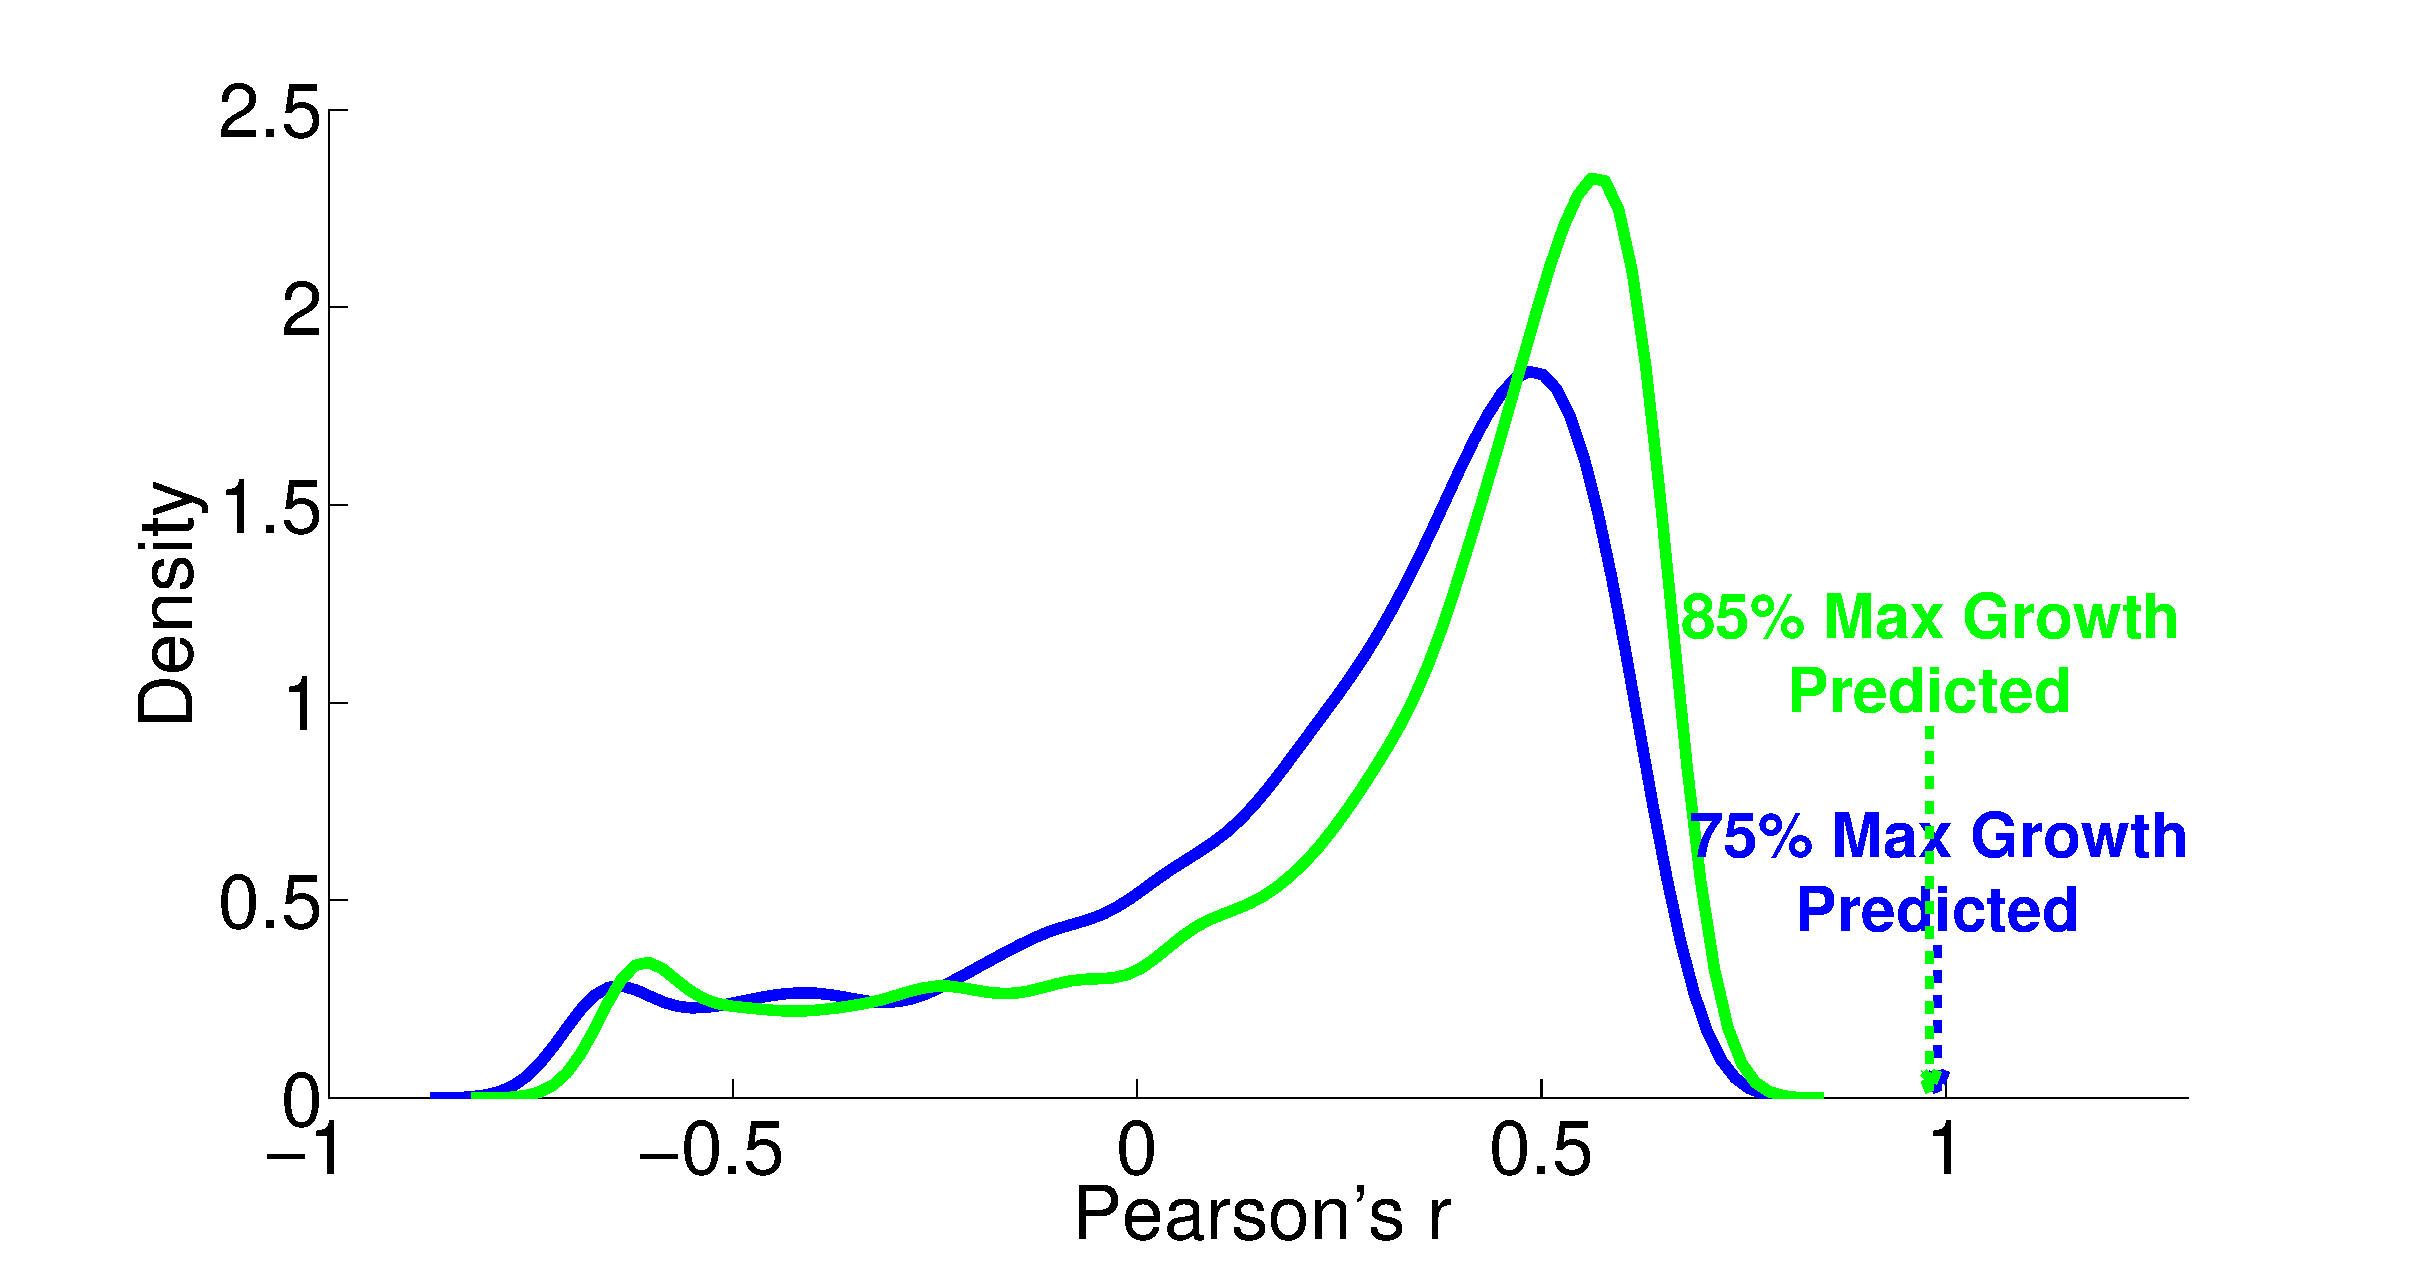
\includegraphics[width=\textwidth]{pExp}
  \caption{Highly constrained.} \label{fig:YpermCorr:A}
  \end{subfigure}
\\
  \begin{subfigure}[b]{0.5\textwidth}
  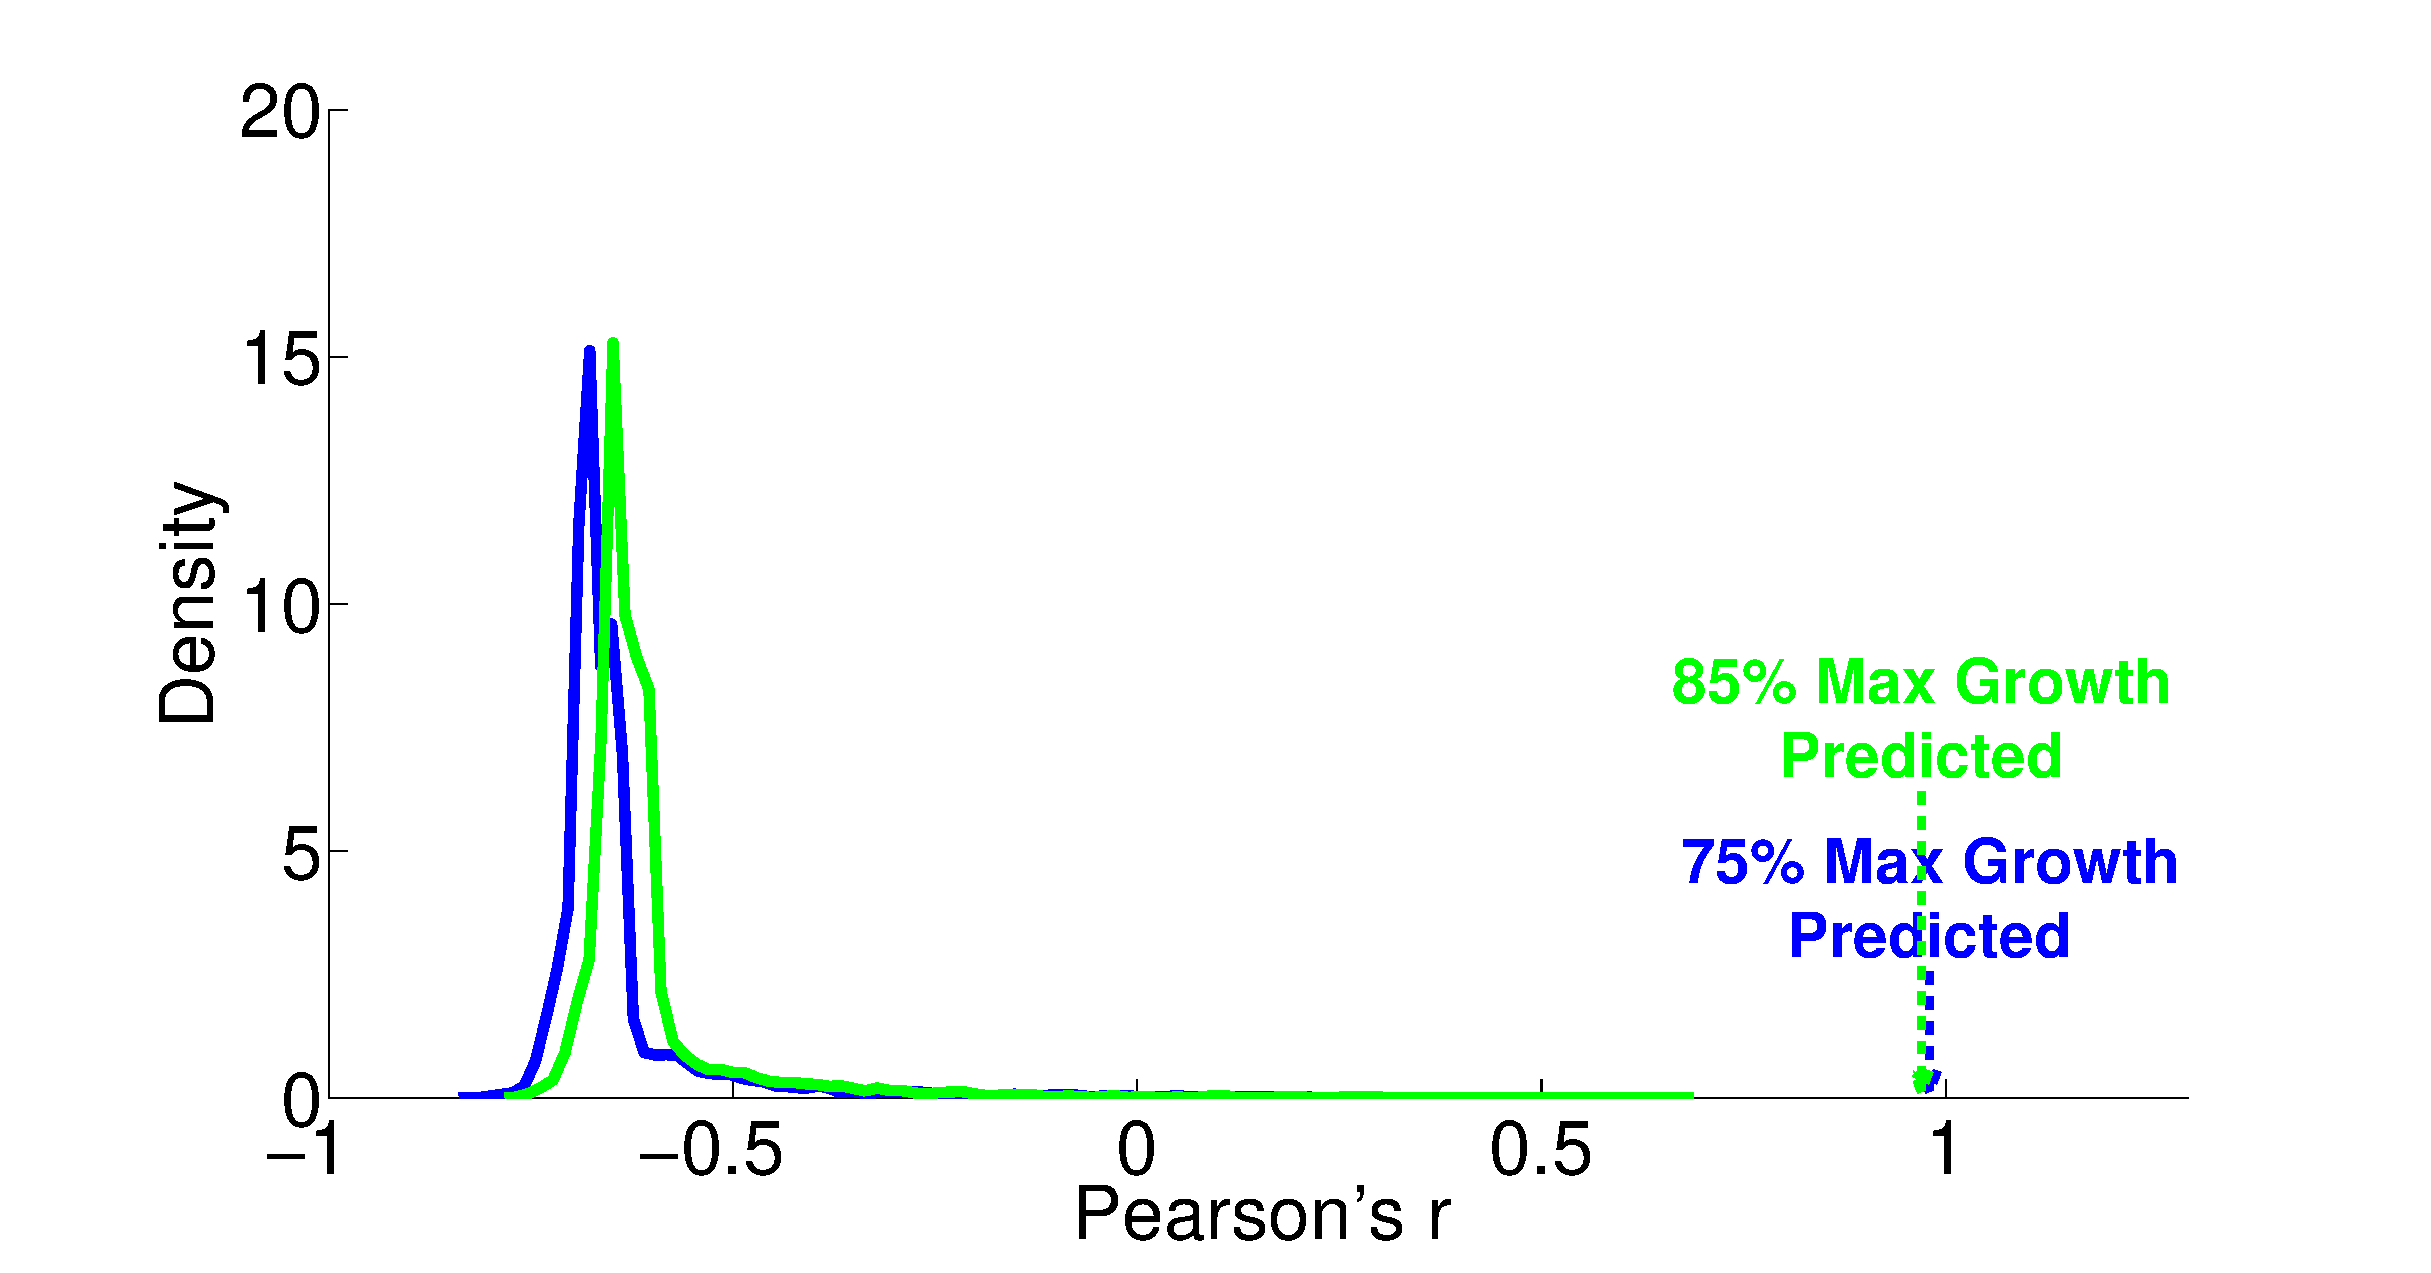
\includegraphics[width=\textwidth]{pExp_dirr}
  \caption{Minimally constrained.} \label{fig:YpermCorr:B}
  \end{subfigure} 
\\
\end{tabular}
\vspace{-4mm} 
\caption{Kernel-smoothed histograms of correlation between
experimental fluxes and fluxes estimated from FALCON when all gene
expression data points are permuted with arrows marking the
correlation when FALCON is run on the unpermuted expression data.}
\label{fig:YpermCorr}
\end{figure}


\subsection{Sensitivity to expression noise}
To understand the sensitivity of flux to expression, we multiply noise
from multivariate log-normal distributions with the expression vector
and see the effect on the estimated fluxes. We find that enzymatic
reaction directionality constraints influence the sensitivity of the
model to expression perturbation (Fig.~\ref{fig:ExpSens}). It is important to
note that mere presence of the constraints does not help us determine
the correct experimental fluxes when other classes of methods (e.g.\
FBA; Table~\ref{tab:FalcPerf}) are used. Additionally, it is possible to obtain
good predictions even without a heavily constrained model (Table~\ref{tab:FalcPerf}).

In order to work with different constraint sets in Yeast, we wrote the
MATLAB function \texttt{removeEnzymeIrrevs} to find all enzymatic
reactions in a model that are annotated as reversible but are
constrained to operate in one direction only. The script then changes
the bounds to allow flux in both directions. The function
\texttt{useYN5irrevs} copies the irreversible annotations found in
Yeast 5.21 \citep{Lee2012} to a newer yeast model, but could in
principle be used for any two models; by default, this script is coded
to first call \texttt{removeEnzymeIrrevs} on both models before
copying irreversible annotations. Application of these scripts removes
853 constraints in Yeast 5.21 and 1,723 constraints in Yeast
7. Despite the significant relaxation in constraints, since nutrient
uptake constraints are unaffected, FBA only predicts a 1.28\%
increase in growth rate in the minimally constrained Yeast 7
model. However, in FALCON, we are no longer optimizing a sink reaction
like biomass, and this relaxation in internal constraints can be more
important (Fig.~\ref{fig:ExpSens}).

\begin{figure}
\centering
\begin{tabular}{c}
  \begin{subfigure}[b]{0.5\textwidth}
  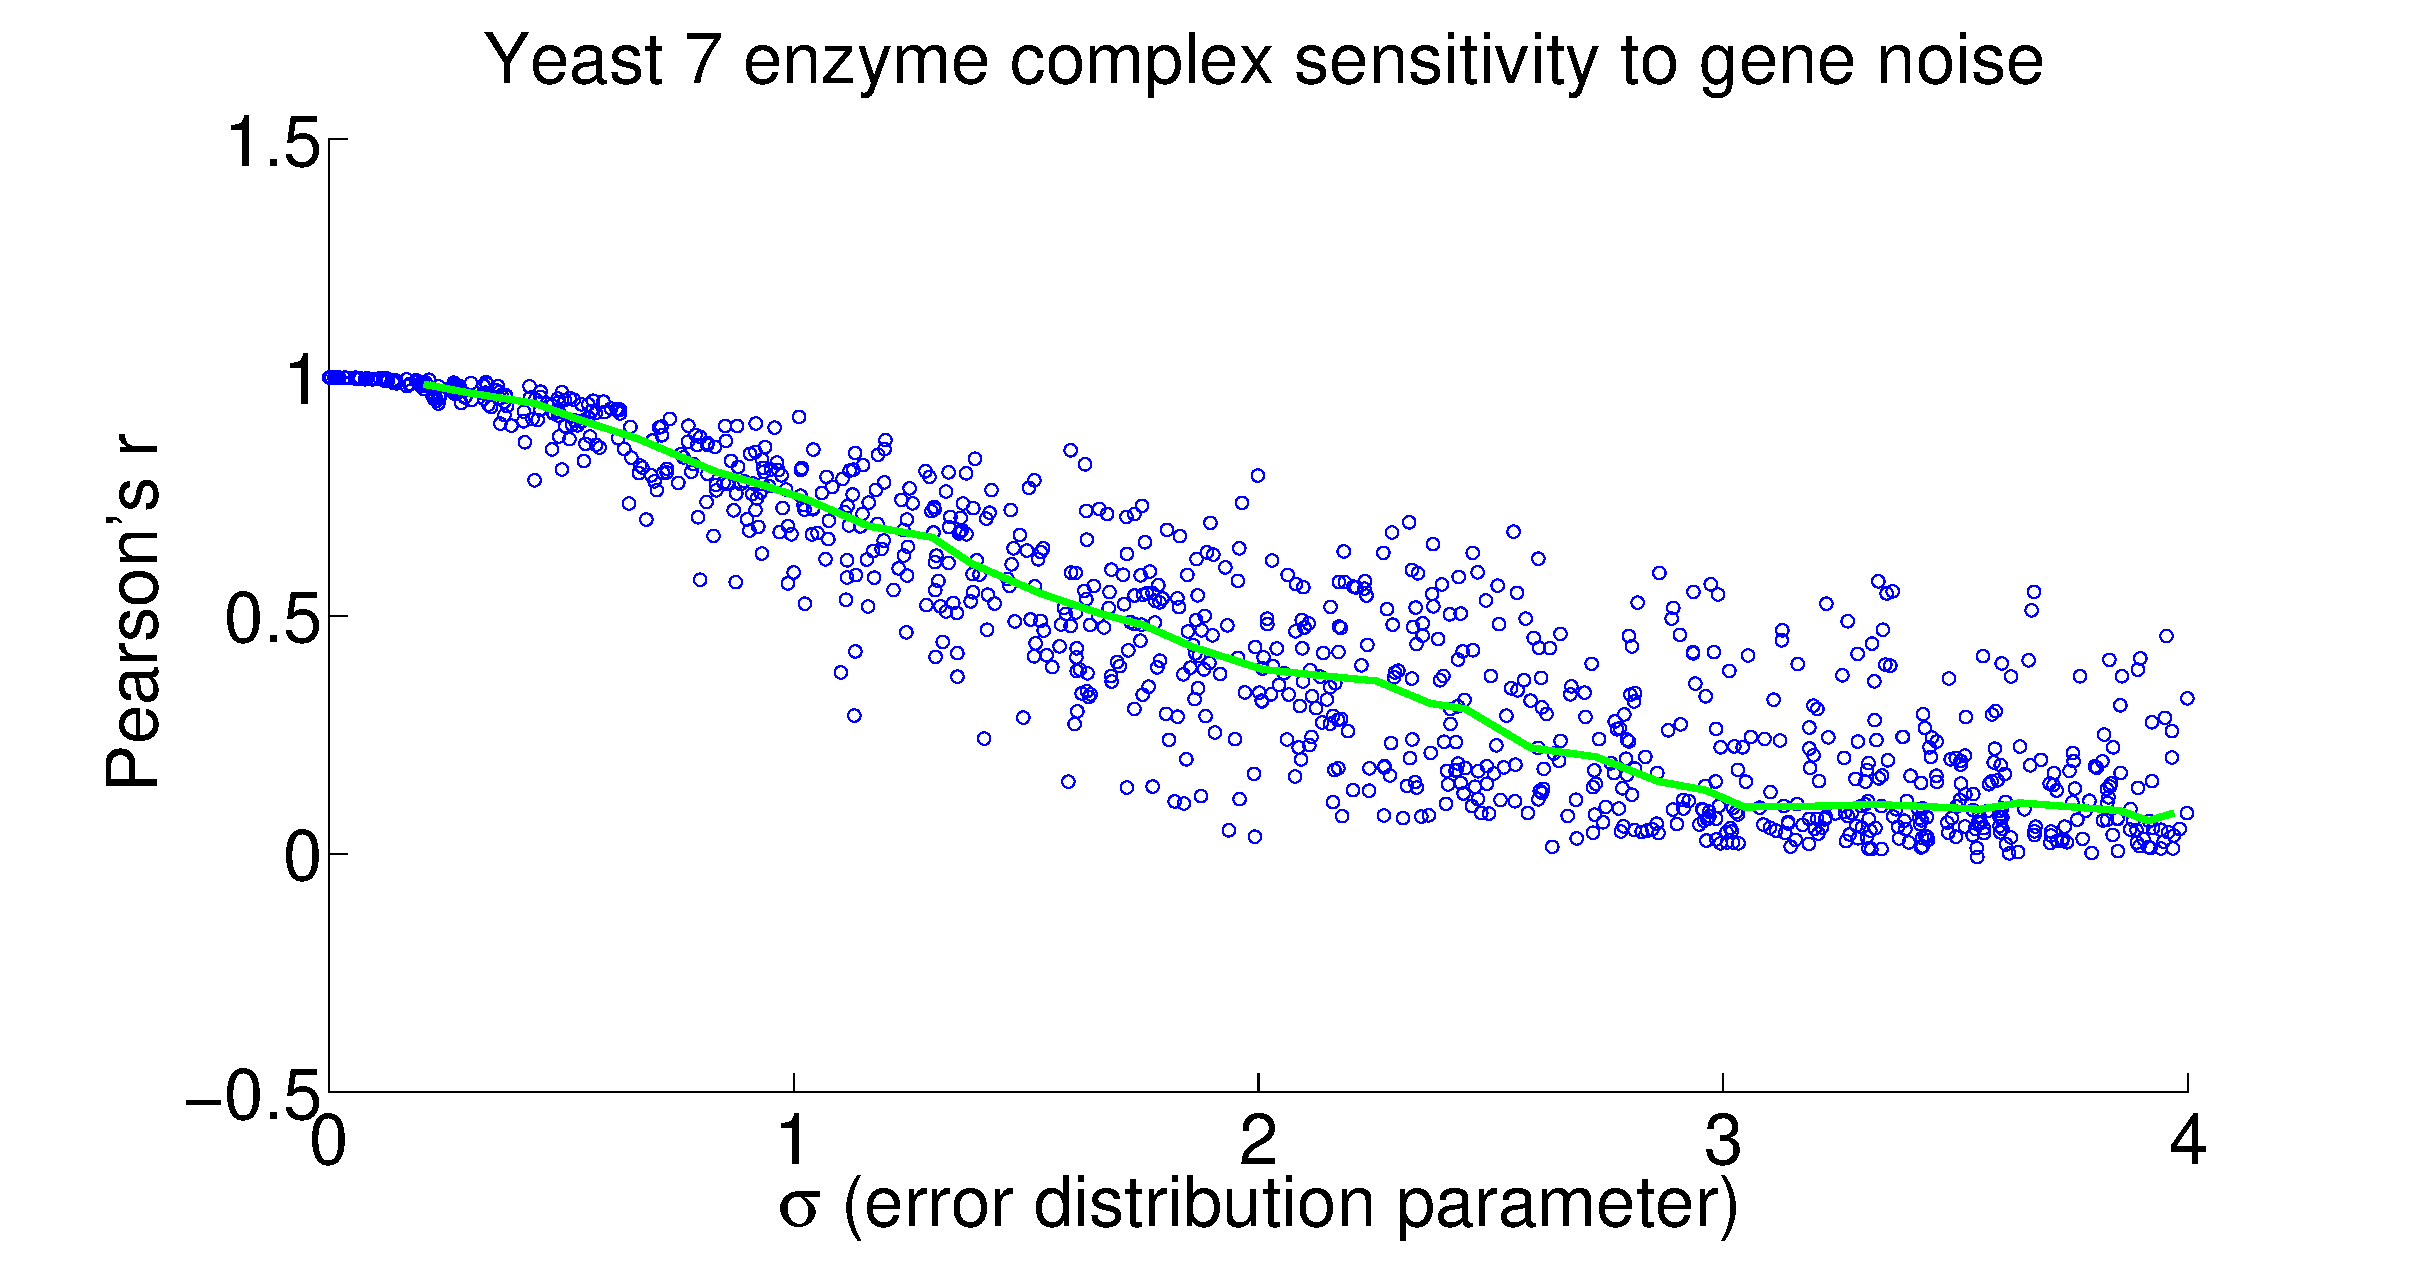
\includegraphics[width=\textwidth]{noise_y7EC}
  \caption{} \label{fig:ExpSens:A}
  \end{subfigure}
\\
  \begin{subfigure}[b]{0.5\textwidth}
  \vspace{-4mm} 
  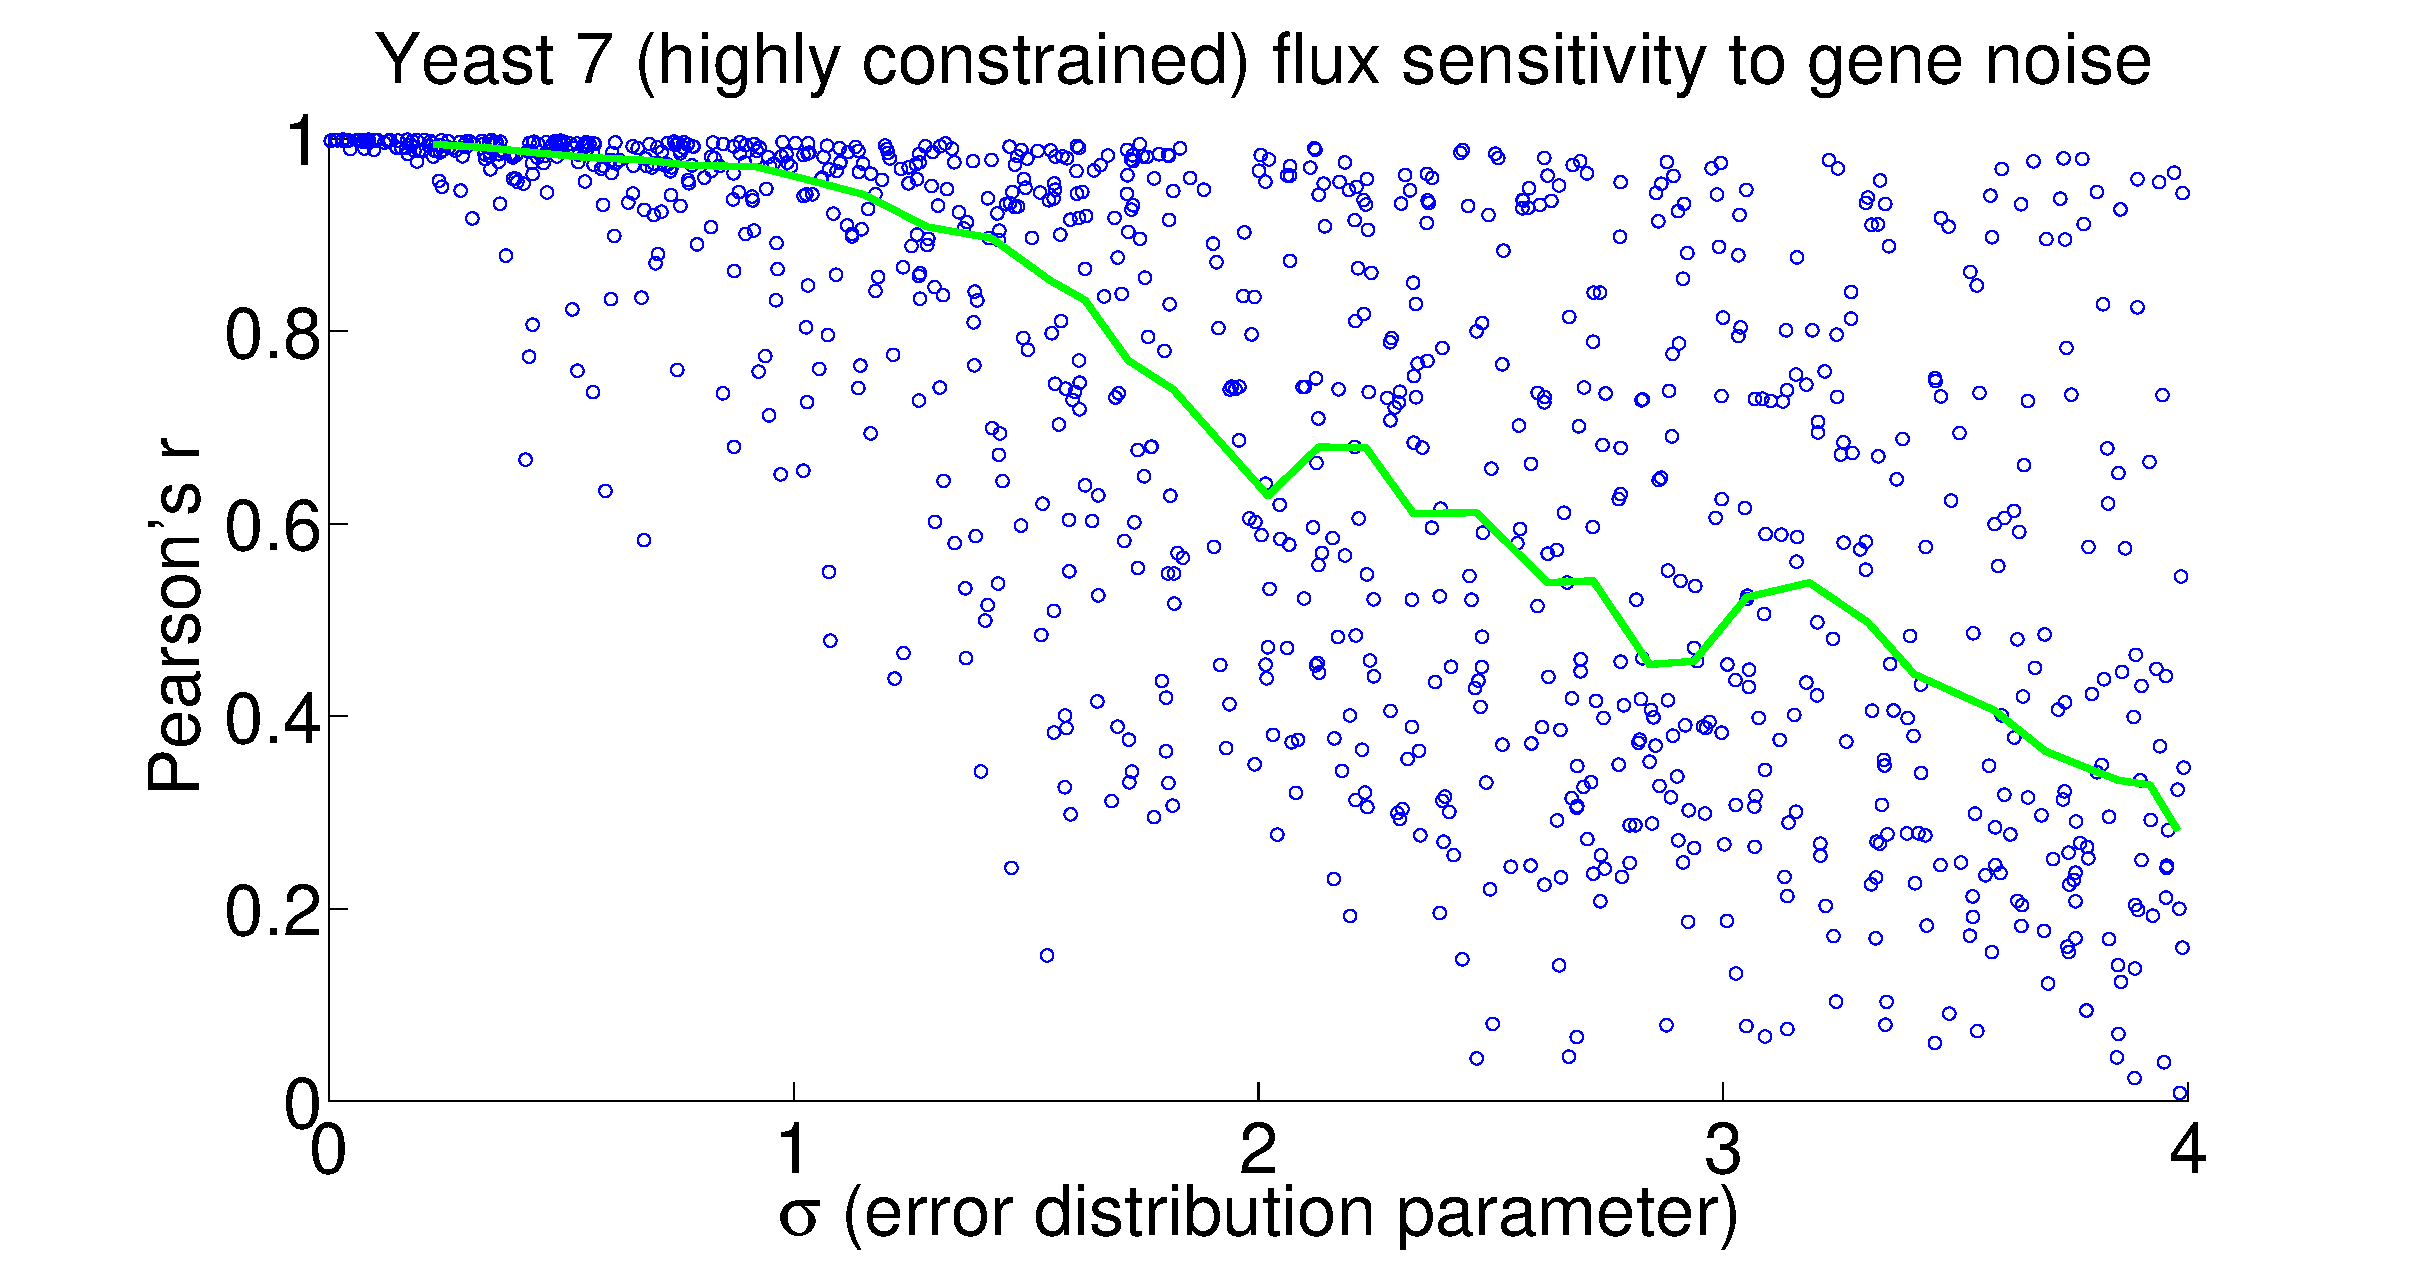
\includegraphics[width=\textwidth]{noise_y7HCflux}
  \caption{} \label{fig:ExpSens:B}
  \end{subfigure} 
\\
  \begin{subfigure}[b]{0.5\textwidth}
  \vspace{-4mm} 
  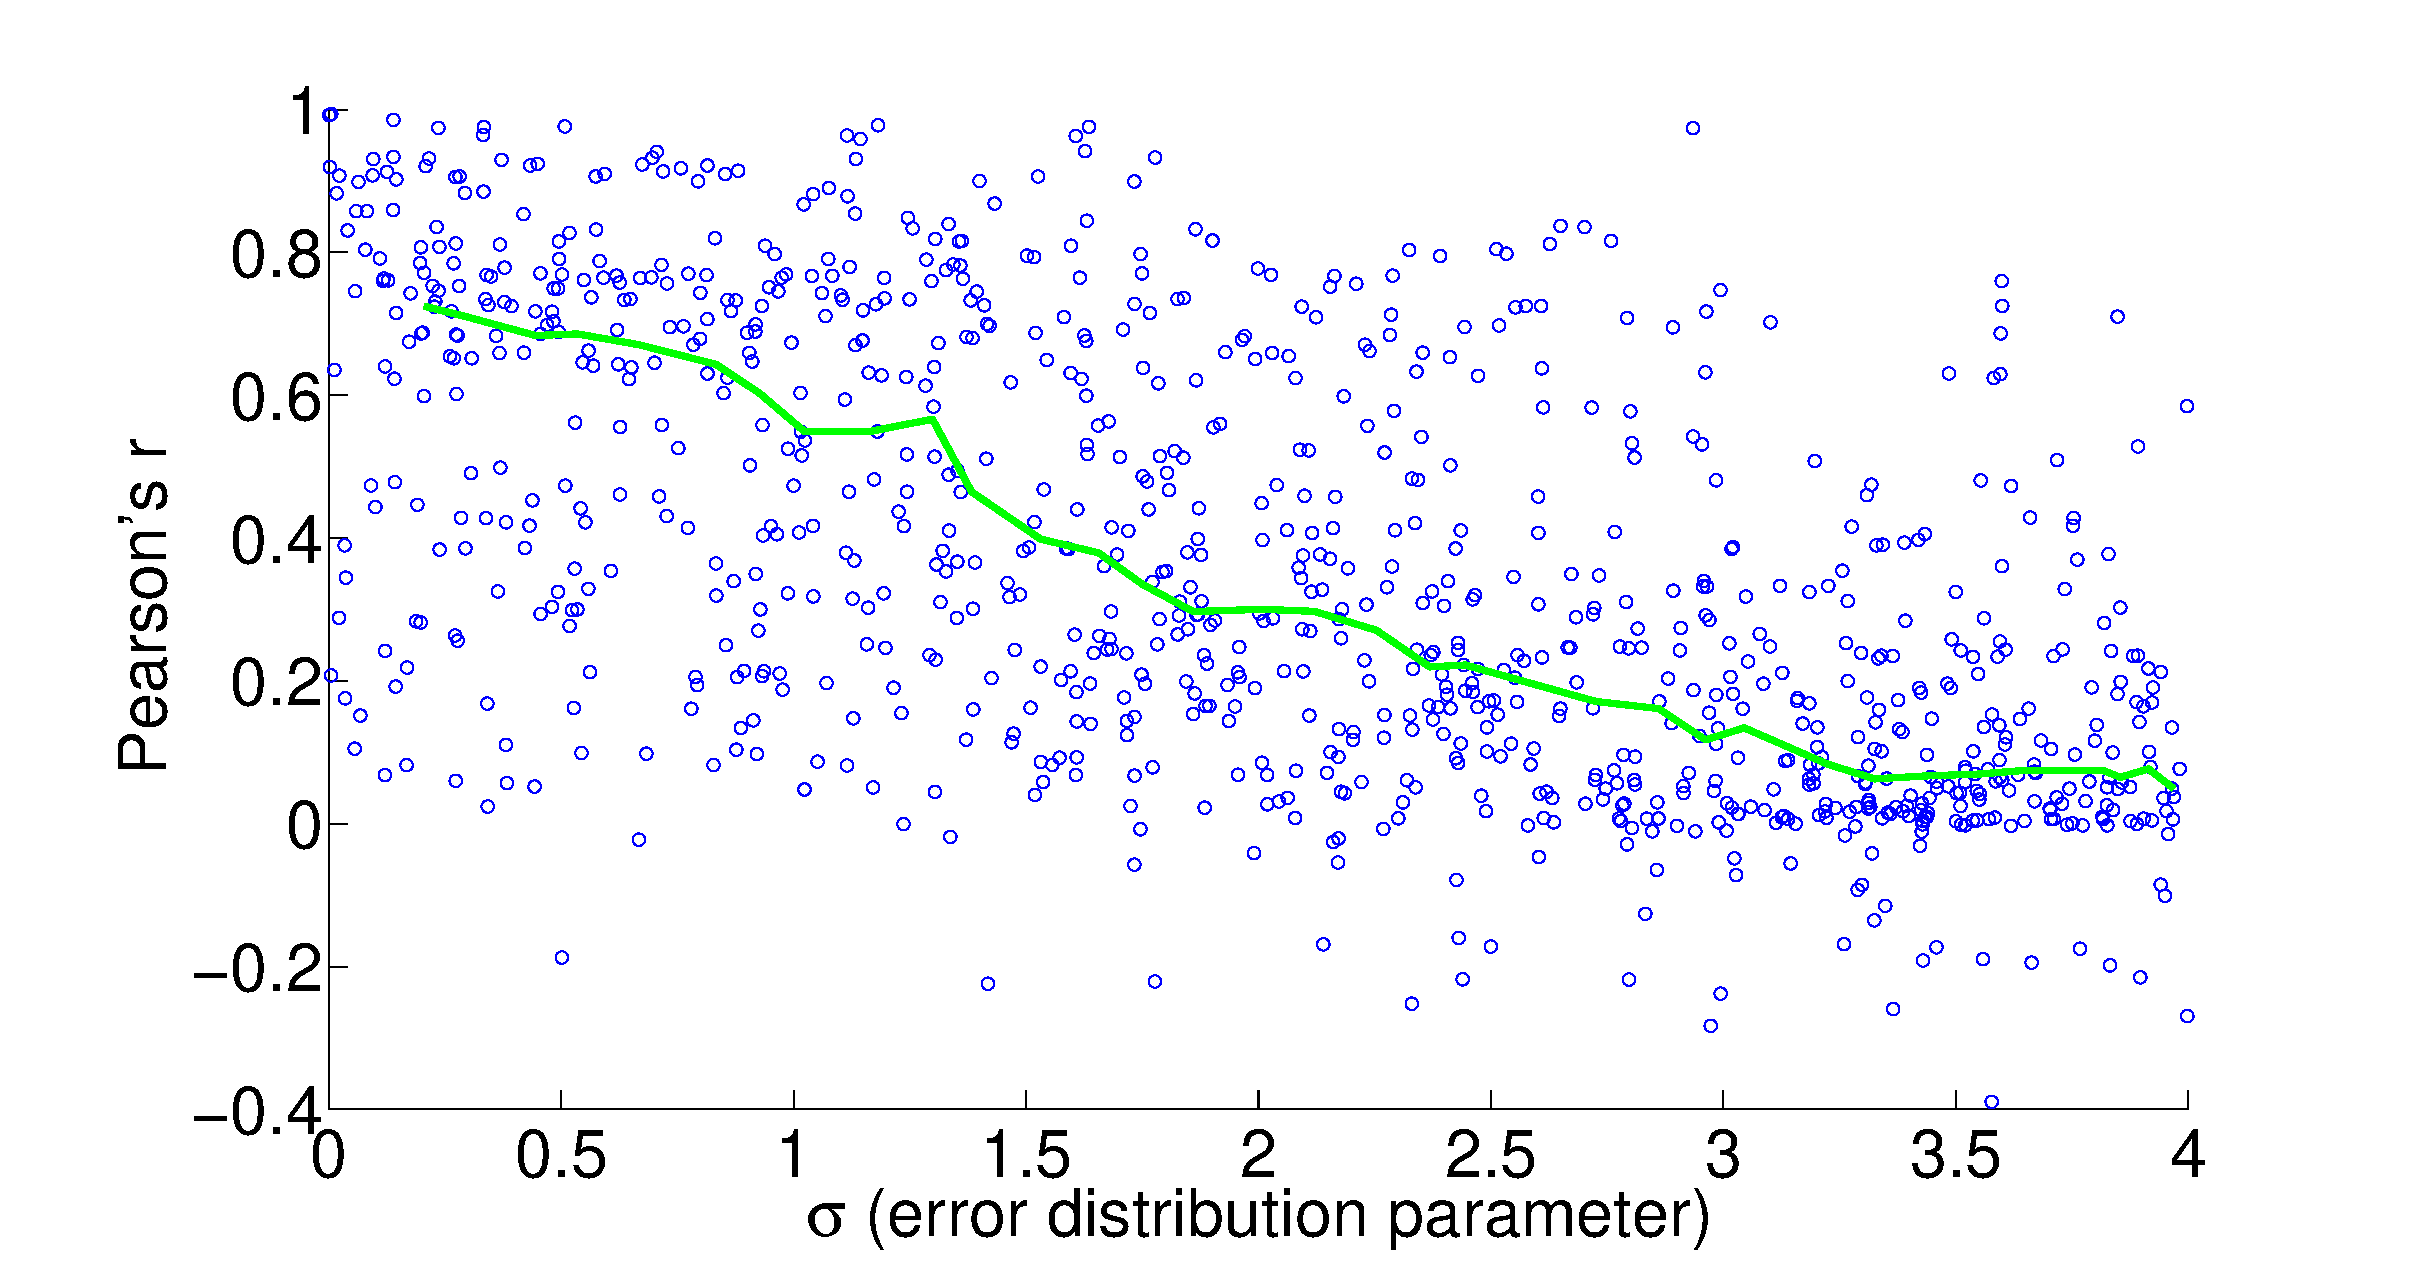
\includegraphics[width=\textwidth]{noise_y7MCflux}
  \caption{} \label{fig:ExpSens:C}
  \end{subfigure} 
\\
\end{tabular}
\vspace{-4mm} 
\caption{
Correlation of perturbed enzyme abundance vectors and flux
vectors with the associated unperturbed vector. The interval median
correlation is shown in green. Noise sampled from a multivariate
log-normal distribution with parameters $\mu=1$ and $\sigma$ (x-axis) is
multiplicatively applied to the enzyme abundance vector, and the
y-axis shows the Pearson correlation between the two vectors
(a). Similar plots shows correlation between flux vectors estimated
with FALCON using the same perturbed and unperturbed expression
vectors (b-c).}
\label{fig:ExpSens}
\end{figure}

For Human Recon 2, additional constraint sets supply some benefit, but
even the most extreme constraint set does not compare to what is
available in Yeast 7, which is also inherently constrained by the fact
that yeast models will be smaller than comparable human models
(\suppOrApp Fig.~\ref{fig:ExpSensRec2}. For
mammalian models, more sophisticated means of constraint, such as
enzyme crowding constraints \citep{Shlomi2011}, or using FALCON in
conjunction with tissue specific modeling tools, may prove highly 
beneficial. For instance, correlation between two types of proteomics
data yields a Pearson's $r = 0.7$ \citep{Gholami2013}, corresponding
to an expected $\sigma \approx 1.4$ and expected $r \approx 0.4$ for
flux in our most highly constrained human model.

\subsection{Flux estimates provides information beyond enzyme complex abundance}
It is not an unreasonable hypothesis that fluxes would correlate well
with their associated complex abundances. Indeed, the general
principle needed for fitting fluxes to enzyme complex abundances is to
assume the values would be correlated in the absence of other
constraints (e.g. branch points that arise from the
stoichiometry). More specifically, it should be the case that flux is
proportional to enzyme complex abundance given ample availability of
substrate, and that this proportionality constant does not vary too
much between reactions.  There are undoubtedly many exceptions to this
rule, but it seems as though there may be some underlying evolutionary
principles for it to work in this parsimonious fashion, as has been
partly verified \citep{Bennett2009}.

Aside from the obvious benefits
of constraint-based methods also estimating fluxes for non-enzymatic
reactions, and assigning a direction for reversible enzymatic
reactions, we see that in general, our method does not predict a
strong correlation between complex abundance and flux
(\suppOrApp Fig.~\ref{fig:FluxExpCmp}). 
Recently it has been shown that many fluxes are not
under direct control of their associated enzyme expression
level \citep{Chubukov2013}, which gives experimental support to the
idea that a network-based approach, such as that
presented in this paper, may be useful in understanding how fluxes may
be constrained by expression data. \citealt{Chubukov2013} also note that enzymes
may be overexpressed in some cases, either for robustness or because
of noise in transcriptional regulation. This will not usually be a
problem in FALCON, unless entire pathways are overexpressed, which
would be unusual as it would represent a seemingly large energetic
inefficiency.

The present work doesn't attempt to use empirically
obtained kinetic parameters to estimate $V_{\max}$, but this approach
does not seem as promising in light of experimental evidence that many
reactions in central carbon metabolism tend to operate well below
$V_{\max}$ \citep{Bennett2009}. Still, a better understanding of these
phenomena may make it possible to improve flux estimation methods such
as the one presented here, or more traditional forms of MFA
\citep{Shestov2013a} by incorporating enzyme complexation and kinetic
information.


\subsection{Increasing roles for GPR rules and complex abundance estimates}
Still, complex abundance may have uses aside from being a first
step in FALCON. The method presented here for complex abundance
estimation can be used as a stand-alone method, as long as GPR
rules from a metabolic reconstruction are present. For instance, it
may not always be desirable to directly compute a flux. As an example,
the relative abundance of enzyme complexes present in secretions
from various biological tissues, such as milk or pancreatic
secretions, may still be of interest even without any intracellular
flux data. Perhaps more importantly, this approach to estimating
relative complex levels can be employed with regulatory models such as
PROM \citep{Chandrasekaran2010a} or other regulatory network models
that can estimate individual gene expression levels at time $t+1$
given the state of the model at a time $t$.

GPR rules and stoichiometry may be inaccurate or
incomplete in any given model. In fact, for the foreseeable future,
this is a given. By using the GPR and not just the stoichiometry to
estimate flux, it is possible that future work could make use of this
framework to debug not just stoichiometry as some methods currently do
(e.g.\ \citealt{Reed14112006}) , but also GPR rules.  Hope for
improved GPR rule annotation may come from many different avenues of
current research. For instance, algorithms exist for reconstructing
biological process information from large-scale datasets, and could be
tuned to aid in the annotation of GPR rules \citep{Mitra2013}. 
Flexible metabolic reconstruction pipelines such as
GLOBUS may also be extended to incorporate GPR rules into their output, and
in so doing, extend this type of modeling to many non-model organisms
\citep{Plata2012}. Another limitation that relates to lack of
biological information is that we always assume a one-to-one copy
number for each gene in a complex. Once more information on enzyme
complex structure and reaction mechanism becomes available, an
extension to the current method could make use of this information.
Even at the current level of structure, we think it is evident
that GPR rules should ungergo some form of standardization;
Boolean rules without negation may not always capture the author's
intent for more complex purposes like flux fitting.



%%%%%%%%%%%%%%%%%%%%%%%%%%%%%%%%%%%%%%%%%%%%%%%%%%%%%%%%%%%%%%%%%%%%%%%%%%%%%%%%%%%%%
%
%     please remove the " % " symbol from \centerline{\includegraphics{fig01.eps}}
%     as it may ignore the figures.
%
%%%%%%%%%%%%%%%%%%%%%%%%%%%%%%%%%%%%%%%%%%%%%%%%%%%%%%%%%%%%%%%%%%%%%%%%%%%%%%%%%%%%%%


\section{Conclusion}

We have formalized and improved an existing method for estimating flux
from expression data, as well as listing detailed assumptions in the
model that may be useful to address in later attempts
\textbf{Table~\ref{tab:ECAssume}}.  Although we show that expression does not
correlate well with flux, we are still essentially trying to fit
fluxes to expression levels.  The number of constraints presents in
metabolic models (even the minimally constrained models) prevents 
a good correlation between the two. However, as
with all constraint-based models, constraints are only half the story in any largely
underdetermined system, and we show that gene expression can prove to
be a valuable basis for forming an objective, as opposed to methods
that continue to use expression to further constrain the model by
creating tissue-specific or condition-specific models
\citep{Shlomi2008,Becker2008}.

For better curated models, the approach described immediately finds
use for understanding metabolism, as well as being a scaffold to find
problems for existing GPR rules, and more broadly the GPR formalism itself.
The present results and avenues for future improvement
show that there is much promise for using expression to estimate
fluxes, and that it can already be a useful tool for performing flux
estimation and analysis.

